
\documentclass[12pt,article]{memoir}

\usepackage{fancyhdr}
\usepackage{graphicx}
\usepackage{fontspec}
\setmainfont{Calibri}
\usepackage{tikz}
\usetikzlibrary{calc}
\usepackage{xcolor}
\usepackage{xpatch}
\usepackage{hyperref}
\usepackage{tabu}
\usepackage{float}
\usepackage{enumerate}

\usepackage[autostyle, english = american]{csquotes}



\usepackage[yyyymmdd]{datetime} % change date format to yyyy/mm/dd to fit ISO8601

\renewcommand{\familydefault}{\sfdefault} % set font
\renewcommand{\dateseparator}{--} % change date-seperators to - to fit ISO8601

\renewcommand\contentsname{Table of Contents}

\chapterstyle{section}
\renewcommand*{\chapnumfont}{\normalfont\HUGE\bfseries\sffamily}
\renewcommand*{\chaptitlefont}{\normalfont\HUGE\bfseries\sffamily}

\makeatletter 
% define macro for itemcode
\newcommand\itemcode[1]{\renewcommand\@itemcode{#1}}
\newcommand\@itemcode{}

% define macro for rev number
\newcommand\revnumber[1]{\renewcommand\@revnumber{#1}}
\newcommand\@revnumber{}
\makeatother

\definecolor{orbitOrange}{RGB}{250,62,0} % the ORBiT orange

\setlrmarginsandblock{2.5cm}{2.5cm}{*}
\setulmarginsandblock{2.5cm}{*}{1}
\checkandfixthelayout 

\setlength{\beforechapskip}{0cm} % reduce chapter spacing

\hypersetup{
    colorlinks,
    citecolor=black,
    filecolor=black,
    linkcolor=black,
    urlcolor=black
}

%**********************************************************************
%Document titles etc. defined here: (replace [] as well)
\title{OA-II VEH Camera System Design}
\author{Jinzhi Cai}
\itemcode{DR00002}
\revnumber{A01}
\date{\today}
%end of document titles etc.
%**********************************************************************

\makeatletter
\let\runtitle\@title
\let\runitemcode\@itemcode
\makeatother

% set header style
\pagestyle{fancy}
{
	\fancyheadoffset{0cm}

	\lhead{\runtitle \ - \runitemcode}
	\rhead{Page: \thepage }
	%\chead{\leftmark} % section name
}

\newcommand{\OrbitBackground}{% For a logo drawn with TikZ
\begin{tikzpicture}[remember picture,overlay] % draw background
	\coordinate (bl) at (current page.south west);
	\coordinate (r) at (current page.east);
    \coordinate (A) at ($(bl)+(0,3cm)$);
    \coordinate (B) at ($(r)+(0,-2cm)$);
    \coordinate (C) at (current page.south east);
    \coordinate (ctrlNode) at ($(current page.south) + (0cm,1cm)$);
    \coordinate (ctrlNode2) at ($(current page.south east) + (-1cm,1cm)$);
    \fill[orbitOrange, fill opacity=0.2]
    (A) .. controls (ctrlNode) and (ctrlNode2) .. (B) -- (C) -- (bl);
    \node [white] at ($(C) + (-3cm,1cm)$) {2015-\the\year \ ORBiT@SU};
\end{tikzpicture}
}

\cfoot{\OrbitBackground}

\begin{document}

\begin{tikzpicture}[remember picture,overlay] % draw background
	\coordinate (bl) at (current page.south west);
	\coordinate (r) at (current page.east);
    \coordinate (A) at ($(bl)+(0,3cm)$);
    \coordinate (B) at ($(r)+(0,-2cm)$);
    \coordinate (C) at (current page.south east);
    \coordinate (ctrlNode) at ($(current page.south) + (0cm,1cm)$);
    \coordinate (ctrlNode2) at ($(current page.south east) + (-1cm,1cm)$);
    \fill[orbitOrange]
    (A) .. controls (ctrlNode) and (ctrlNode2) .. (B) -- (C) -- (bl);
    \node [white] at ($(C) + (-3cm,1cm)$) {2015-\the\year \ ORBiT@SU};
\end{tikzpicture}

\makeatletter

\includegraphics[width=\textwidth]{../logo.jpg}\\[4ex]
\begin{center}
	\bfseries \fontsize{50}{50}\selectfont  \@title \\[2ex]
	\LARGE  \@itemcode
\end{center}
\vfill
\begin{flushright}
	\LARGE Rev: \@revnumber\\
	\large \@author\\
	\large \@date\\[18ex]
\end{flushright}
\makeatother
\thispagestyle{empty}
\newpage

\tableofcontents*
\thispagestyle{fancy}
\newpage

%**********************************************************************
% Everything after this is the main document. Edit below this line,

\chapter{Introduction}
\section{Scope}
This document discuss the current camera technology and construct a design that will fulfill the need for OA-II VEH system.
\section{Purpose}
The goal for this document is come up with a design that will provide four 1080p 60Hz video steam and storage to a central storage media by research the current camera technology.
\chapter{Revision History}

\begin{table}[H]
	\centering
	\resizebox{0.8\textwidth}{!}{%
		\begin{tabu}{r || c | c | c }
		Rev\# & Editor & Delta & Date\\ \hline
		A01 & Jinzhi Cai & Initialize & 2019-7-10\\
		\end{tabu}
	}
	\caption{Summary of Revision History}
	\label{tab:rev}
\end{table}

\newpage
\chapter{General Structure of Camera System}
\section{Introduction}
The most basic camera system have three part. The camera sensor is the device that will receive data from the environment and transfer it via the camera interface. The data that flow out from the sensor is call raw data. It contain all the information that the camera get from the environment. A 1080p 60Hz camera have $1920*1080=2073600 pixels$. One pixels usually take $3 Bytes$ to save. For each second, $2073600*3*60=373248000Bytes$ will be created. That will be $355.96MB/s$ for one single camera.The encoder is use to compress the video steam smaller for it to transmission via long distence data link(usually with in $1MB/s$). The storage unit is use to save the video steam to a file and allow future replay.
\begin{figure}[htp]
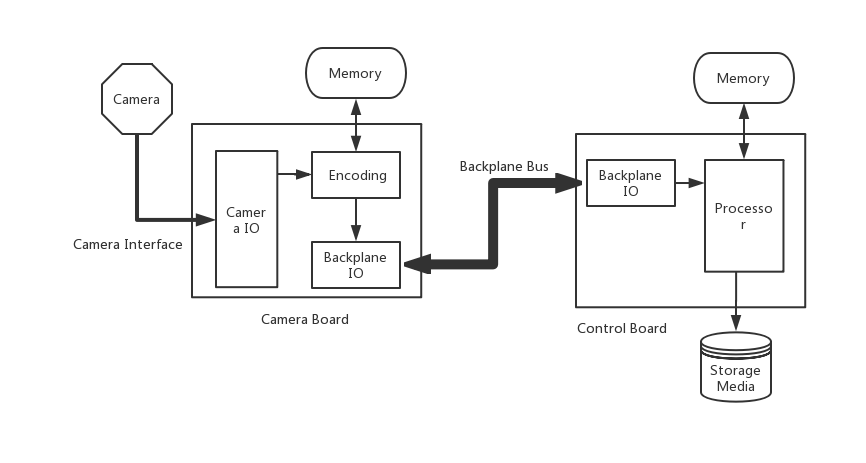
\includegraphics[width=\textwidth]{DR00002_GenDia.png}
 \caption{General Structure of Camera System}	
\end{figure}
\newpage
%
%**********************************************************************
\chapter{Camera Sensor and Relative Interface}
\section{Introduction}
The camera sensor is the most improtant part in the camera system. The classic camera interface is use the same way to output the video signal as a monitor do. For each pixel clock, data of a pixel is been sended. After few clock(depend on the resolution), Line Sync rise to indecate one line data is finish transmission. The Frame Sync is indecate a frame of pixel data is sended. However, modern camera sensor usually use one of those three camera interface. Some of the is samiliar with the classic one, and other improve it.\\\\\
\begin{figure}[htp]
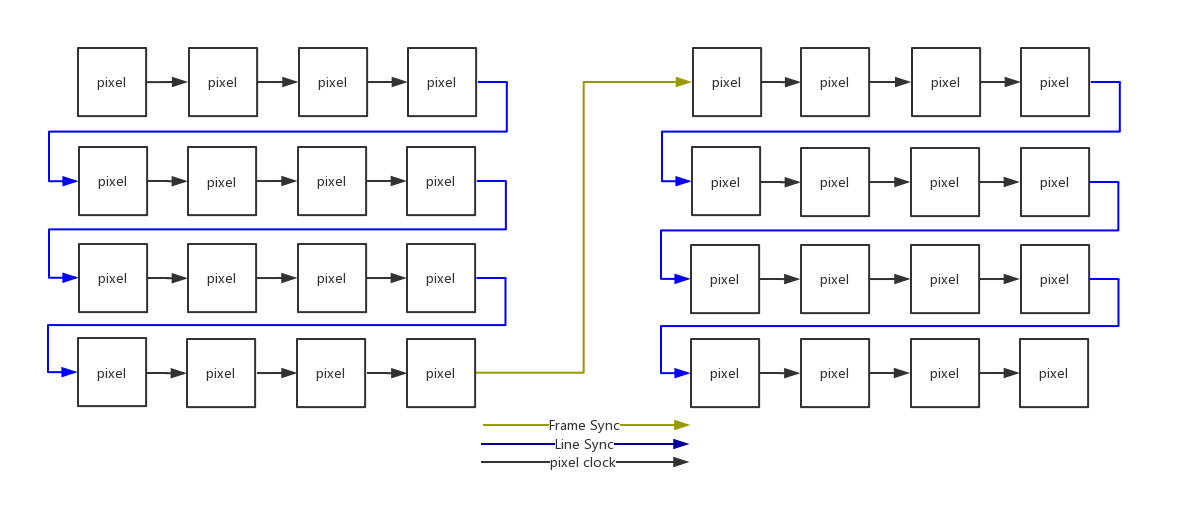
\includegraphics[width=\textwidth]{DR00002_Cam.png}
 \caption{Classic Video Stream}	
\end{figure}
\newpage
\section{DVP Interface} 
The DVP interface is use the classic video interface to transmit data out from the sensor. The I2C bus(SCK, SDA) that inside the interface is use to config the camera. The main clock is use to provide a clock for the camera. The VSYNC, HSYNC, PCLK is the clock system that help processor to indecate the weight and height of frame. The D OUT is data that comming out from the camera. It have low requirement on the trace and sample interface design. However, it can not offer long distence transmission and high speed clock. It usually use at low end 240p camera.
\begin{figure}[htp]
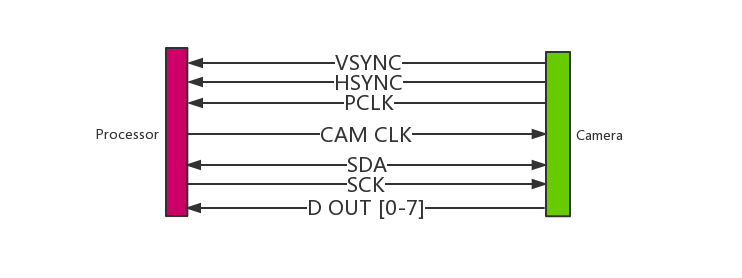
\includegraphics[width=\textwidth]{DR00002_DVP.png}
 \caption{Physical Layer for DVP Interface}	
\end{figure}
\begin{description}
	\item[\textbf{D OUT}]Data out put
	\item[\textbf{VSYNC}]Lane Sync Signal
	\item[\textbf{HSYNC}]Frame Sync Signal
	\item[\textbf{PCLK}]Pixel Clock
	\item[\textbf{CAM CLK}]Main Camera Clock
	\item[\textbf{SDA}]I2C Data Line
	\item[\textbf{SCK}]I2C Clock Line
\end{description}
\newpage
\section{LVDS Interface}
The LVDS camera interface is use LVDS technology to improve classic DVP interface. It use differential signal to transmitting data. It increase the lane it need to send data, but differential signal can prevent common mode interference which limit the DVP clock for increasing.
\begin{figure}[htp]
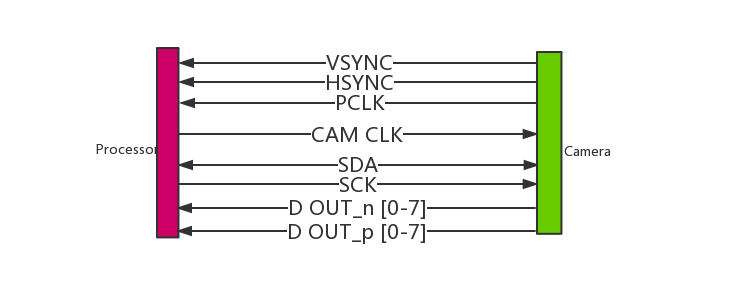
\includegraphics[width=\textwidth]{DR00002_LVDS.png}
 \caption{Physical Layer for LVDS Interface}	
\end{figure}
\begin{description}
	\item[\textbf{DOUT n/p}]Differential Data Lane
	\item[\textbf{VSYNC}]Lane Sync Signal
	\item[\textbf{HSYNC}]Frame Sync Signal
	\item[\textbf{PCLK}]Pixel Clock
	\item[\textbf{CAM CLK}]Main Camera Clock
	\item[\textbf{SDA}]I2C Data Line
	\item[\textbf{SCK}]I2C Clock Line
\end{description}
\newpage
\section{MIPI CSI-2 Interface}
The MIPI CSI-2 camera inferface$\footnote{Might only avaliable in high-end chip.}$ is different from the old one. The goal for this bus is to cut down the lane count for camera module and allow more data flow to the processor. In structure, the MIPI CSI-2 camera interface use different way to communicate. The MIPI interface use package as the data communication unit. Inside the sensor, data will be pack into a package and send it via the two or four data lane. The same process will reverse and output the raw camera data. MIPI camera will allow 1080p 60Hz or 4K 30Hz.  
\begin{figure}[htp]
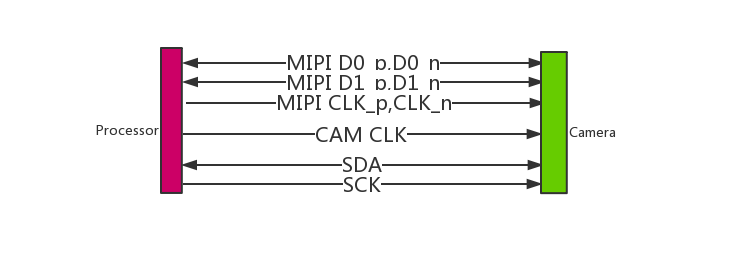
\includegraphics[width=\textwidth]{DR00002_MIPI.png}
 \caption{Physical Layer for 2 Lane MIPI Interface}	
\end{figure}
\begin{description}
	\item[\textbf{MIPI D0n/p}]MIPI Data Lane 0
	\item[\textbf{MIPI D1n/p}]MIPI Data Lane 1
	\item[\textbf{MIPI CLKn/p}]MIPI Clock
	\item[\textbf{CAM CLK}]Main Camera Clock
	\item[\textbf{SDA}]I2C Data Line
	\item[\textbf{SCK}]I2C Clock Line
\end{description}
\section{USB Interface (UVC)}
The USB camera interface$\footnote{It do have success example by using ZYNQ SoC FPGA.}$ is different with the rest of the interface. In those camera, it include DSP chip that already finish the video compression. It is easy to use but do not support 60fps.
\newpage
%**********************************************************************
\chapter{Camera Interface Bridge Chip}
\section{Lattice CrossLink}
The CrossLink is Lattice made small scale MIPI bridge FPGA.$\footnote{Too small for hardware encoder}$ It include two MIPI D-PHY and up to 8 mipi data lane. It also support interface translation (MIPI CSI-2 -> DVP).
\begin{figure}[htp]
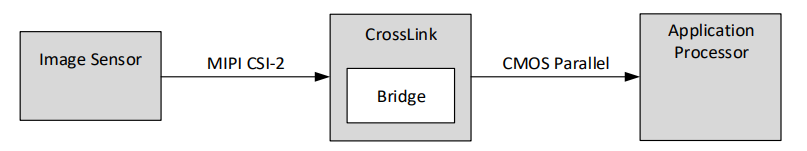
\includegraphics[width=\textwidth]{DR00002_CrossLink.png}
 \caption{Block Diagram for CrossLink}	
\end{figure}
\section{Toshiba Camera Interface Bridge}
The Toshiba Camera Interface Bridge is a stand alone chip that can converse MIPI CSI-2 bus to DVP bus. It also offer I2C bus to configure chip setting.
\begin{figure}[h]
\begin{center}
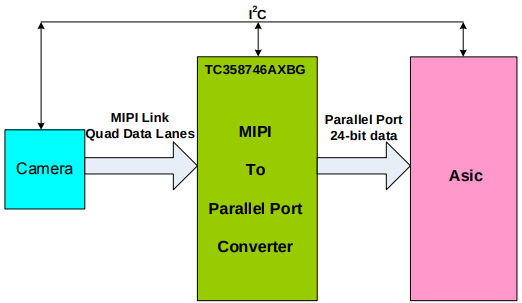
\includegraphics[width=0.7\textwidth]{DR00002_Toshiba.png}
 \caption{Block Diagram for Toshiba}	
 \end{center}
\end{figure}
\newpage
%**********************************************************************
\chapter{H.264 Video Steam Encoding}
\section{Introduction}
The H.264 Encoder is another important unit in the camera system. Due to the data flow of a camera sensor is too much for the backplane bus, compression is nessary.
\section{IP Core Description}
\subsection{SoC Technology}
This IP core fit for both \textbf{Intel} and \textbf{Xilinx}
\begin{table}[H]
	\centering
		\begin{tabu}{r || c | c | c }
		Version & LUT use & Test Platform & Price for Platform\\ \hline
		Standard Version & 110k & Zynq-7 Z7045 & \$1000\\
		Slim Version & 50k & Artix-7 XC7A200T & \$300\\
		I-Frame Version & 45k & Spartan-6 LX150 & \$200\\
		\end{tabu}
	\caption{SoC Summary}
	\label{tab:socs}
\end{table}
\subsection{A2E Technology}
\begin{table}[H]
	\centering
		\begin{tabu}{r || c | c | c }
		Version & LUT use & Test Platform & Price for Platform\\ \hline
		Xilinx(1080p 30Hz) & 11K & Zynq-7 Z7020 & \$300\\
		Xilinx(1080p 60Hz) & 11K & Kintex-7 & \$500\\
		Xilinx(1080p 180Hz) & 11K & Zynq UltraScale & \$1000\\\hline
		%*************************************************************%
		Intel(1080p 30Hz) & 8K & Cyclone V SoC & \$500\\
		\end{tabu}
	\caption{SoC Summary}
	\label{tab:socs}
\end{table}
\newpage
\section{Encoding SoC Chip}
\subsection{HiSilicon Hi3559}
Hi3559 is HiSilicon made new generation mobile camera soc. It support MIPI interface and H.264 Video encoding up to 1080P 60Hz. It can output video via USB 2.0 bus.\\\\
\begin{figure}[htp]
\begin{center}
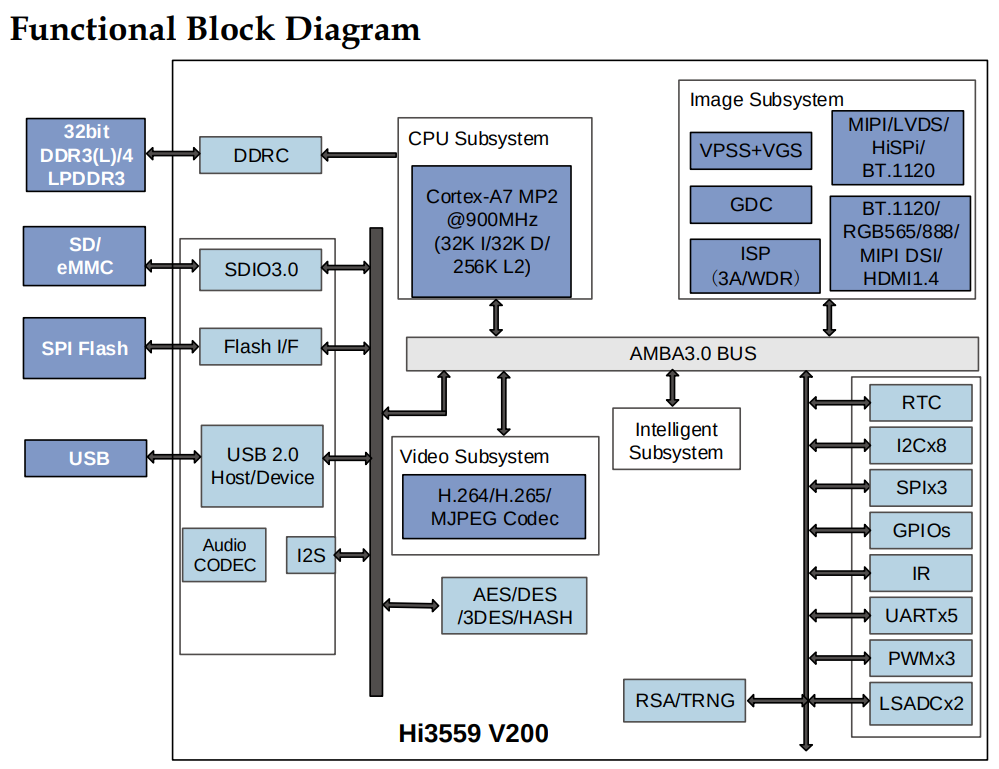
\includegraphics[width=\textwidth]{DR00002_Hi3559.png}
 \caption{Block Diagram for Hi3559}	
\end{center}
\end{figure}
\newpage
\subsection{OmniVision OV798}
OV798 is OmniVision made camera soc. It support MIPI interface and H.264 Video encoding up to 720P 60Hz. It can output video via USB 2.0 bus.\\\\
\begin{figure}[htp]
\begin{center}
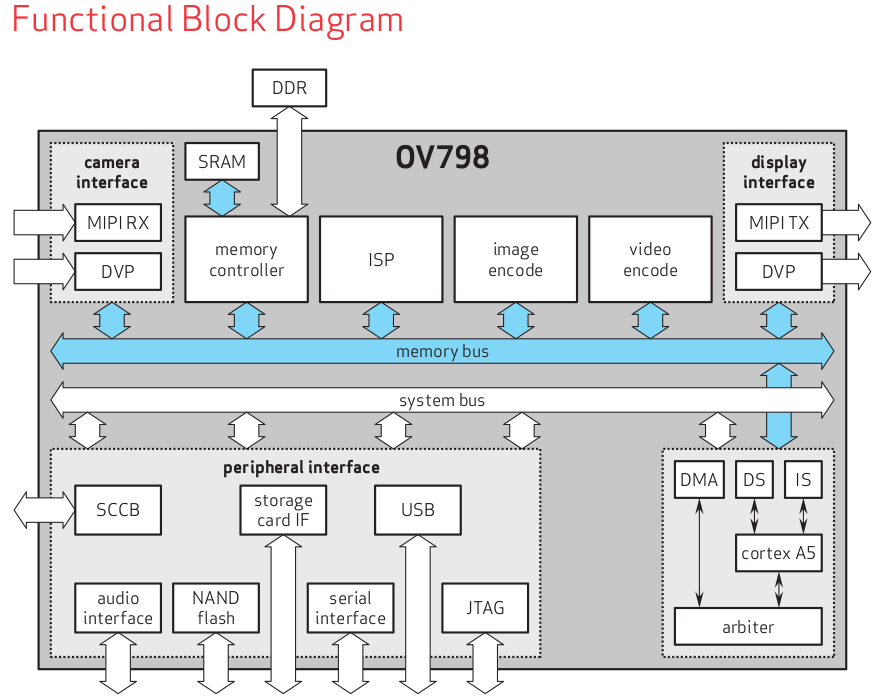
\includegraphics[width=\textwidth]{DR00002_Omni.png}
 \caption{Block Diagram for OV798}	
\end{center}
\end{figure}
\newpage
%**********************************************************************
\chapter{File System and Video Storage}
\section{Introduction}
\section{Comparsion}
\begin{table}[H]
	\centering
		\begin{tabu}{r || c | c | c | c }
		Technology & Interface & Speed & Complexity & Price\\ \hline
		SSD Drive & NVMe & 800MB/s & 9 &  \$1000/500GB\\
		SSD Drive & SATA & 715MB/s & 9 & \$500/500GB \\
		eMMC & eMMC & 45MB/s & 5 & \$10/128G \\
		SD Card & SDIO & 80MB/s & 5 & \$15/64G \\
		\end{tabu}
	\caption{SoC Summary}
	\label{tab:socs}
\end{table}
\newpage
%**********************************************************************
\chapter{System Diagram}
\newpage
%end of document
%**********************************************************************
\end{document}
